\chapter{Chimie verte et procédés industriels}\label{ch:b3:green-industrial}

L'ibuprofène était autrefois fabriqué en six étapes qui rejetaient plus de
masse qu'elles n'en conservaient~: sels d'aluminium, chlorure de sodium,
éthanol, ammoniac et acide acétique quittaient l'usine pour chaque
kilogramme de médicament. Depuis 1992, une voie catalytique en trois étapes
transforme en produit la plupart des atomes qu'elle utilise, et son seul
sous-produit, l'acide acétique, est récupéré et vendu. Ce chapitre chiffre
de telles comparaisons~: \omterm{def:b3:green-industrial:atom-economy}{économie d'atomes}, \omterm{def:b3:green-industrial:e-factor}{facteurs E} et \omterm{def:b3:green-industrial:pmi}{intensité
massique du procédé}~; il examine ensuite les solvants, l'énergie et
l'\omterm{def:b3:green-industrial:lca}{analyse du cycle de vie}, la façon dont certains des plus grands procédés
chimiques ont été rendus plus propres, et ce que changent les \omterm{def:b3:green-industrial:feedstock}{matières
premières renouvelables} et les \omterm{def:b3:complex-kinetics:enzyme}{enzymes}.

\begin{recall}
Le volume scolaire a introduit l'\omterm{def:b3:green-industrial:atom-economy}{économie d'atomes} et la \omterm{def:b3:green-industrial:green-chemistry}{chimie verte}~; le
volume de première année, les rendements~; le volume de deuxième année, les
réacteurs, le taux de conversion, la sélectivité, le temps de séjour, la
conversion par passage, le recyclage et la purge, l'élévation adiabatique
de température, les électrolyseurs et les piles à combustible. Le
\cref{ch:b3:surfaces-catalysis} et le \cref{ch:b3:homogeneous-catalysis}
ont traité la catalyse, le \cref{ch:b3:total-synthesis} les mesures d'une
voie de synthèse.
\end{recall}

\begin{omfigure}
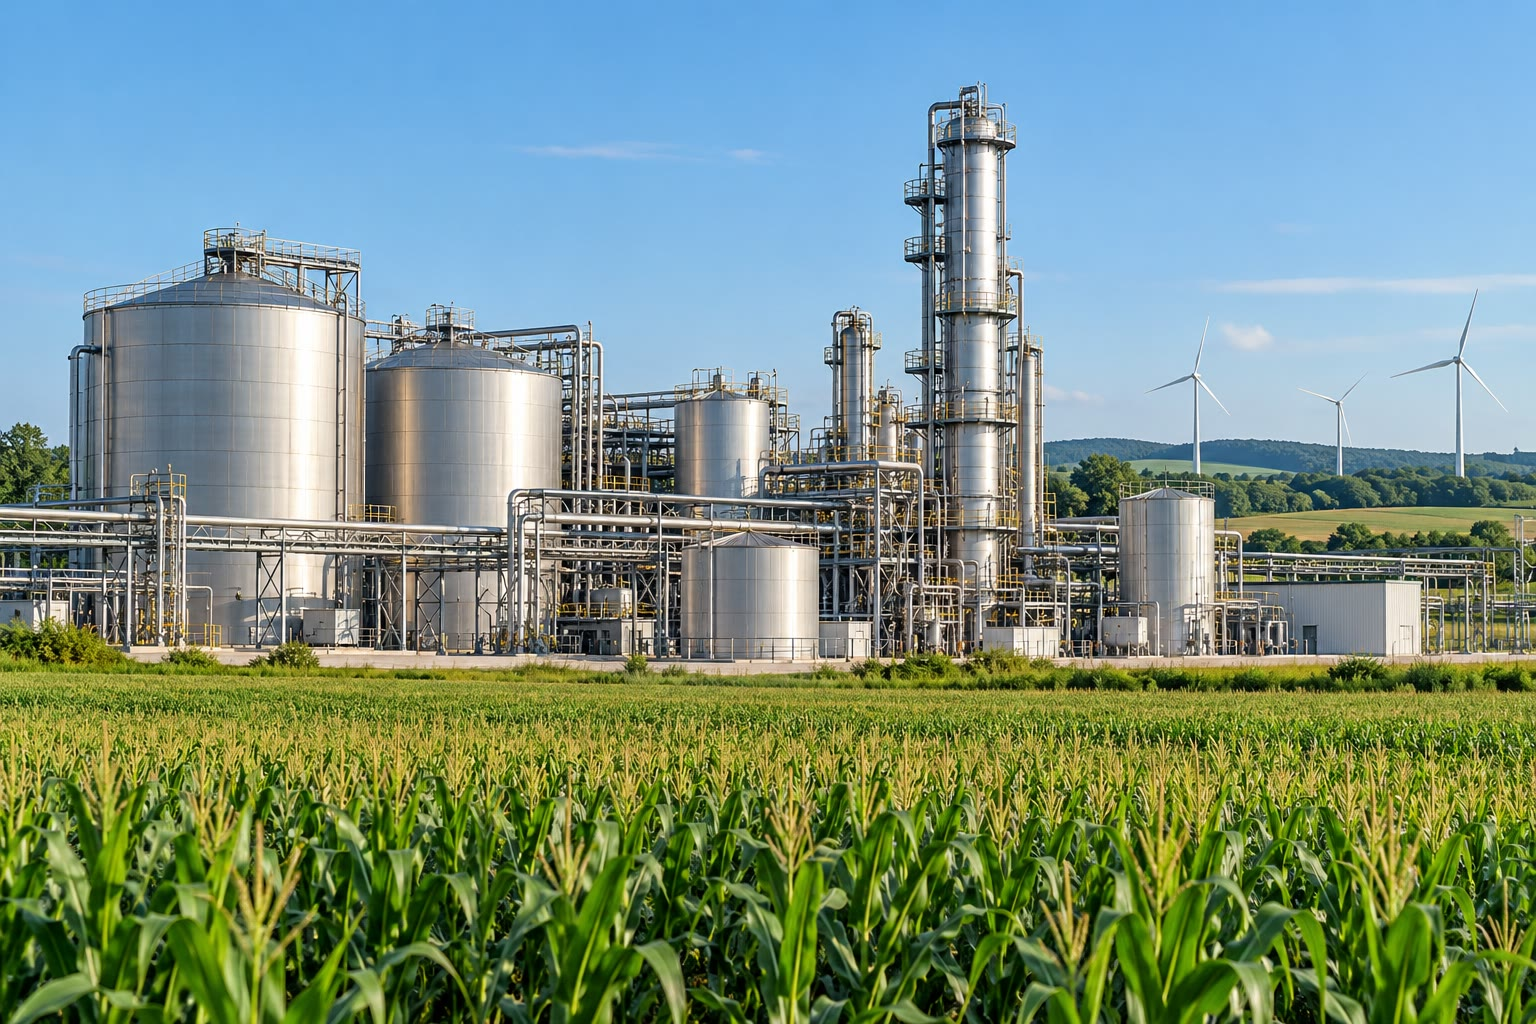
\includegraphics[width=0.58\linewidth]{images/book4/ai/b3-31-biorefinery.jpg}

{\small Une bioraffinerie~: des cuves de fermentation et une colonne de
distillation qui transforment cultures et résidus en carburants et en
\omterm{def:b3:green-industrial:feedstock}{molécules plateformes}.}
\end{omfigure}

\section{Mesurer le caractère vert}

\begin{definition}[Chimie verte]\label{def:b3:green-industrial:green-chemistry}
La \emph{chimie verte}\index{chimie verte} est la conception de produits et
de procédés chimiques qui réduisent ou éliminent l'utilisation et la
production de substances dangereuses, résumée en douze principes~:
prévenir les déchets, maximiser l'\omterm{def:b3:green-industrial:atom-economy}{économie d'atomes}, utiliser et produire
des substances moins dangereuses, concevoir des produits plus sûrs,
utiliser des solvants plus sûrs, économiser l'énergie, utiliser des
\omterm{def:b3:green-industrial:feedstock}{matières premières renouvelables}, éviter les dérivés inutiles, préférer les
catalyseurs aux réactifs stœchiométriques, concevoir pour la dégradation,
surveiller en temps réel, et choisir une chimie intrinsèquement plus sûre.
\end{definition}

\begin{definition}[Économie d'atomes]\label{def:b3:green-industrial:atom-economy}
L'\emph{économie d'atomes}\index{economie d'atomes@économie d'atomes} d'une réaction est la masse molaire
du produit voulu divisée par la somme des masses molaires de tous les
réactifs de l'équation équilibrée, exprimée en pourcentage.
\end{definition}

\begin{proposition}[Économie d'atomes par classe de réactions]\label{prop:b3:green-industrial:ae-classes}
Les additions et les réarrangements ont une \omterm{def:b3:green-industrial:atom-economy}{économie d'atomes} de 100\,\%~;
les substitutions et les éliminations, moins.
\end{proposition}

\begin{proof}
Dans une addition, $\mathrm{A} + \mathrm{B} \to \mathrm{AB}$, ou un réarrangement, $\mathrm{A} \to \mathrm{A'}$, l'unique produit contient tous les
atomes des réactifs, si bien que sa masse molaire est égale à la somme des
leurs. Une substitution, $\mathrm{A{-}X} + \mathrm{Y} \to \mathrm{A{-}Y} + \mathrm{X}$, ou une élimination, $\mathrm{A} \to \mathrm{B} + \mathrm{C}$, produit un
second produit qui emporte de la masse.
\end{proof}

\begin{definition}[Facteur E]\label{def:b3:green-industrial:e-factor}
Le \emph{facteur E}\index{facteur E} d'un procédé est la masse de déchets par
masse de produit. Dans le facteur E complet, toutes les entrées qui ne
finissent pas dans le produit comptent comme déchets, solvants et eau
compris~; le facteur E simple exclut les solvants et l'eau.
\end{definition}

\begin{definition}[Intensité massique du procédé]\label{def:b3:green-industrial:pmi}
L'\emph{intensité massique du procédé}\index{intensite massique du procede@intensité massique du procédé} (PMI) est la masse
totale des matières introduites dans un procédé (réactifs, auxiliaires,
solvants, eau) par masse de produit.
\end{definition}

\begin{proposition}[PMI et facteur E]\label{prop:b3:green-industrial:pmi-e}
Pour un même périmètre, $\mathrm{PMI} = E + 1$, avec $E$ le \omterm{def:b3:green-industrial:e-factor}{facteur E} complet.
\end{proposition}

\begin{proof}
Par conservation de la masse, tout ce qui entre ressort soit comme produit, soit comme déchet~:
$m_{\mathrm{in}} = m_{\mathrm{product}} + m_{\mathrm{waste}}$. La division par $m_{\mathrm{product}}$ donne $\mathrm{PMI} = 1 + E$.
\end{proof}

\begin{definition}[Efficacité massique de réaction]\label{def:b3:green-industrial:rme}
L'\emph{efficacité massique de réaction}\index{efficacite massique de reaction@efficacité massique de réaction} (RME) d'une
réaction est la masse de produit obtenue divisée par la masse totale des
réactifs utilisés.
\end{definition}

\begin{proposition}[RME, rendement et économie d'atomes]\label{prop:b3:green-industrial:rme}
$\mathrm{RME} = \mathrm{AE} \times \text{rendement}/\mathrm{SF}$, où le facteur stœchiométrique $\mathrm{SF} \ge 1$ est la masse de
réactifs utilisés divisée par la masse qu'exige l'équation équilibrée.
\end{proposition}

\begin{proof}
Pour une mole de produit attendue, l'équation exige une masse $\sum M_r$ de réactifs et
l'essai en utilise $\mathrm{SF}\sum M_r$~; il donne $\text{rendement} \times M_{\mathrm p}$ de produit. En divisant~:
$\mathrm{RME} = \text{rendement}\,M_{\mathrm p}/(\mathrm{SF}\sum M_r) = \mathrm{AE} \times \text{rendement}/\mathrm{SF}$.
\end{proof}

\begin{method}[Calculer les indicateurs d'une voie]\label{met:b3:green-industrial:metrics}
\begin{enumerate}
  \item Écrire l'équation équilibrée de chaque étape et calculer
        l'\omterm{def:b3:green-industrial:atom-economy}{économie d'atomes} de la voie à partir de tous les réactifs qui y
        entrent.
  \item À partir du dossier de lot, additionner les masses de tout ce qui
        est chargé (réactifs, auxiliaires, solvants, eau, matières du
        traitement)~: PMI = total entré / produit.
  \item $E = \mathrm{PMI} - 1$~; soustraire les flux récupérés et réutilisés s'ils sont à l'intérieur du
        périmètre, et le préciser.
  \item RME pour chaque étape~: produit / réactifs, pour trouver où la
        matière se perd (faible rendement, excès de réactif ou mauvaise
        \omterm{def:b3:green-industrial:atom-economy}{économie d'atomes}).
\end{enumerate}
\end{method}

\begin{omfigure}
\begin{tikzpicture}
\begin{axis}[name=a, width=0.48\linewidth, height=5.4cm, ybar, bar width=14pt, ymin=0, ymax=110,
  xtick={1,2,3,4}, xticklabels={{ibuprofène, 6 étapes}, {ibuprofène, 3 étapes}, {OE, chlorhydrine}, {OE, directe}},
  x tick label style={font=\scriptsize, rotate=25, anchor=north east}, ylabel={économie d'atomes / \%},
  axis lines=left, tick label style={font=\scriptsize}, label style={font=\small},
  nodes near coords, nodes near coords style={font=\scriptsize, /pgf/number format/fixed, /pgf/number format/precision=0},
  enlarge x limits=0.18]
\addplot[fill=omMeth!55, draw=omMeth] table[x=i, y=AE] {figdata/out/bachelor-3-green-metrics.dat};
\end{axis}
\begin{axis}[at={(a.east)}, anchor=west, xshift=1.4cm, width=0.48\linewidth, height=5.4cm, ybar, bar width=14pt, ymin=0, ymax=3.4,
  xtick={1,2,3,4}, xticklabels={{ibuprofène, 6 étapes}, {ibuprofène, 3 étapes}, {OE, chlorhydrine}, {OE, directe}},
  x tick label style={font=\scriptsize, rotate=25, anchor=north east}, ylabel={facteur E minimal},
  axis lines=left, tick label style={font=\scriptsize}, label style={font=\small},
  nodes near coords, nodes near coords style={font=\scriptsize, /pgf/number format/fixed, /pgf/number format/precision=2},
  enlarge x limits=0.18]
\addplot[fill=omThm!45, draw=omThm] table[x=i, y=Emin] {figdata/out/bachelor-3-green-metrics.dat};
\end{axis}
\end{tikzpicture}

{\small \omterm{def:b3:green-industrial:atom-economy}{Économies d'atomes} de deux voies vers l'ibuprofène et de deux voies
vers l'oxyde d'éthylène (OE), et plus petits \omterm{def:b3:green-industrial:e-factor}{facteurs E} qu'elles permettent
(tous les rendements à 100\,\%, sans solvant)~:
$E_{\min} = (1 - \mathrm{AE})/\mathrm{AE}$. Les \omterm{def:b3:green-industrial:e-factor}{facteurs E} réels, avec des rendements inférieurs à 100\,\%, des
excès de réactifs et des solvants, sont plus grands.}
\end{omfigure}

\section{Solvants et énergie}

Les solvants représentent en général la plus grande part de la masse d'un
procédé de chimie fine ou pharmaceutique. Les guides de choix des solvants
les classent selon des critères de sécurité, de santé et d'environnement~:
l'eau, l'éthanol, l'acétate d'éthyle, le 2-méthyltétrahydrofurane et
l'anisole sont recommandés~; le dichlorométhane, le chloroforme, le
benzène, l'hexane, le diméthylformamide et le 1,4-dioxane sont à éviter ou
interdits. L'eau, le dioxyde de carbone supercritique (qui dissout les
composés apolaires et ne laisse aucun résidu quand on relâche la pression)
et les réactions sans solvant suppriment le problème à la source.

\begin{method}[Utiliser un guide de choix des solvants]\label{met:b3:green-industrial:solvent-choice}
\begin{enumerate}
  \item Lister ce que le solvant doit faire~: dissoudre les réactifs,
        résister aux réactifs, bouillir à une température utilisable, se
        séparer de l'eau lors du traitement.
  \item Choisir d'abord dans la classe recommandée~; vérifier ses mentions
        de danger.
  \item Si un solvant problématique est nécessaire, chercher un solvant
        recommandé de même fonction (le 2-méthyltétrahydrofurane à la place
        du dichlorométhane ou du THF dans les extractions, l'acétate
        d'éthyle et l'heptane à la place de l'hexane en chromatographie).
  \item Prévoir sa récupération par distillation, et compter ce qui est
        perdu dans le \omterm{def:b3:green-industrial:e-factor}{facteur E}.
\end{enumerate}
\end{method}

\begin{definition}[Intensification des procédés]\label{def:b3:green-industrial:intensification}
L'\emph{intensification des procédés}\index{intensification des procedes@intensification des procédés} est la
reconception des équipements et des conditions opératoires pour rendre un
procédé beaucoup plus petit, plus sûr ou plus efficace~: réacteurs à flux
continu de faible volume et de grande surface d'échange thermique,
distillation réactive, chauffage par micro-ondes.
\end{definition}

Dans un réacteur à flux continu, seul un faible volume d'un intermédiaire
dangereux existe à chaque instant, et la chaleur est évacuée bien plus vite
que dans une grande cuve en discontinu~; des réactions qui s'emballeraient
dans une cuve peuvent être menées à plus haute température et à plus forte
concentration. Les catalyseurs remplacent les réactifs stœchiométriques,
ce qui économise à la fois le réactif et le déchet qu'il devient~:
l'acylation de Friedel--Crafts de l'ancienne voie de l'ibuprofène utilisait
le chlorure d'aluminium en quantité stœchiométrique, détruit lors du
traitement~; la nouvelle utilise le fluorure d'hydrogène comme catalyseur
et comme solvant, récupéré et réutilisé.

\section{Raisonner en cycle de vie}

\begin{definition}[Analyse du cycle de vie]\label{def:b3:green-industrial:lca}
Une \emph{analyse du cycle de vie}\index{analyse du cycle de vie} (ACV) évalue les
impacts environnementaux d'un produit sur toute sa vie, de l'extraction des
matières premières à l'élimination. Elle s'exprime par \emph{unité fonctionnelle}\index{unite fonctionnelle@unité fonctionnelle},
le service rendu (par exemple, un lavage d'une charge de linge), à
l'intérieur d'une \emph{frontière du système}\index{frontiere du systeme@frontière du système} qui précise les
procédés inclus. Une \emph{évaluation du berceau à la porte}\index{evaluation du berceau a la porte@évaluation du berceau à la porte}
s'arrête quand le produit quitte l'usine.
\end{definition}

\begin{omfigure}
\begin{tikzpicture}[font=\scriptsize, >=Stealth,
  box/.style={draw, rounded corners, fill=omDef!10, align=center, minimum height=8mm, inner sep=3pt}]
  \node[box] (r) at (0,0) {extraction\\ des matières\\ premières};
  \node[box] (p) at (2.6,0) {production\\ chimique};
  \node[box] (f) at (5.2,0) {formulation,\\ emballage};
  \node[box] (u) at (7.8,0) {usage};
  \node[box] (e) at (10.2,0) {fin de vie~:\\ recyclage,\\ élimination};
  \foreach \a/\b in {r/p, p/f, f/u, u/e} \draw[->, thick] (\a) -- (\b);
  \draw[omThm, thick, dashed, rounded corners] (-1.1,-0.75) rectangle (3.75,0.75);
  \node[omThm, anchor=north] at (1.3,-0.8) {frontière du berceau à la porte};
  \draw[omMeth, thick, dashed, rounded corners] (-1.25,-1.35) rectangle (11.5,0.95);
  \node[omMeth, anchor=north] at (5.1,-1.4) {frontière du berceau à la tombe};
  \node[anchor=south] at (5.1,1.0) {entrées~: matières, énergie, eau \quad sorties~: produit, émissions, déchets};
\end{tikzpicture}

{\small Étapes de la vie d'un produit et deux \omterm{def:b3:green-industrial:lca}{frontières du système}. Les
entrées et les sorties sont inventoriées pour chaque procédé situé à
l'intérieur de la frontière et converties en catégories d'impact
(changement climatique, acidification, consommation d'eau,
toxicité\dots) par \omterm{def:b3:green-industrial:lca}{unité fonctionnelle}.}
\end{omfigure}

\begin{definition}[Empreinte carbone]\label{def:b3:green-industrial:carbon-footprint}
L'\emph{empreinte carbone}\index{empreinte carbone} d'un produit est son
émission de gaz à effet de serre sur son cycle de vie, exprimée en masse
de dioxyde de carbone ayant le même effet de réchauffement.
\end{definition}

\begin{method}[Mettre en place une ACV comparative]\label{met:b3:green-industrial:lca}
\begin{enumerate}
  \item Énoncer l'objectif et l'\omterm{def:b3:green-industrial:lca}{unité fonctionnelle}~: comparer ce qui rend
        le même service, non la même masse.
  \item Tracer la même \omterm{def:b3:green-industrial:lca}{frontière du système} pour les deux options.
  \item Inventorier les entrées et les sorties de chaque procédé situé à
        l'intérieur, avec les sources et les dates des données.
  \item Convertir en catégories d'impact, puis chercher les compromis
        (moins de carbone mais plus d'eau) et tester la sensibilité de la
        conclusion aux données.
\end{enumerate}
\end{method}

\section{Grands procédés et leur amélioration}

\begin{proposition}[Le dioxyde de carbone de l'ammoniac]\label{prop:b3:green-industrial:smr}
Fabriquer l'ammoniac avec du dihydrogène issu du vaporeformage du méthane
libère, du seul fait de la matière première,
$3/8$ mole de $\ce{CO2}$ par mole de $\ce{NH3}$~: environ \qty{0.97}{t} de $\ce{CO2}$ par tonne d'ammoniac.
\end{proposition}

\begin{proof}
Le vaporeformage suivi de la réaction du gaz à l'eau s'écrit globalement $\ce{CH4 + 2H2O -> CO2 + 4H2}$. La synthèse
s'écrit $\ce{N2 + 3H2 -> 2NH3}$~: deux moles d'ammoniac exigent trois moles de dihydrogène, soit $3/4$ mole de
méthane et $3/4$ mole de $\ce{CO2}$~; par mole d'ammoniac, $3/8$. Une tonne d'ammoniac
(\qty{17.0}{g/mol}) représente $\qty{5.88e4}{mol}$, ce qui donne $\qty{2.21e4}{mol} \times \qty{44.0}{g/mol} = \qty{0.97}{t}$ de $\ce{CO2}$. La combustion du méthane
qui fournit la chaleur du vaporeformage en ajoute davantage.
\end{proof}

% ledger: nh3:world-2024
Les usines d'ammoniac, qui produisent environ 150 millions de tonnes
d'azote par an, comptent parmi les plus grandes sources ponctuelles de
dioxyde de carbone industriel~; le dihydrogène issu de l'électrolyse
alimentée par une électricité bas carbone, ou le captage du carbone au
reformeur, sont les voies pour la réduire. La boucle de synthèse de
l'ammoniac elle-même, avec sa faible conversion par passage, le recyclage
du gaz qui n'a pas réagi et la purge de l'argon et du méthane qui
s'accumuleraient sinon, est déjà efficace.

\begin{omfigure}
\begin{tikzpicture}[font=\scriptsize, >=Stealth,
  box/.style={draw, rounded corners, fill=omMeth!10, align=center, minimum height=8mm, inner sep=3pt}]
  \node[box] (m) at (0,0) {mélangeur};
  \node[box] (c) at (2.6,0) {compresseur};
  \node[box] (r) at (5.2,0) {convertisseur\\ (catalyseur au fer)};
  \node[box] (s) at (8.0,0) {condenseur,\\ séparateur};
  \draw[->, thick] (-1.8,0) -- (m) node[pos=0, left, align=right] {$\ce{N2 + 3H2}$\\ (appoint)};
  \draw[->, thick] (m) -- (c); \draw[->, thick] (c) -- (r); \draw[->, thick] (r) -- (s);
  \draw[->, thick] (s) -- ++(0,-1.2) node[below] {$\ce{NH3}$ liquide};
  \draw[->, thick] (s.north) -- ++(0,0.8) -| node[pos=0.25, above] {recyclage du gaz n'ayant pas réagi} (m.north);
  \draw[->, thick, omThm] ($(s.north)+(0,0.8)$) -- ++(1.6,0) node[right] {purge (Ar, $\ce{CH4}$)};
\end{tikzpicture}

{\small La boucle de synthèse de l'ammoniac~: le gaz frais est mélangé au
gaz recyclé, comprimé et envoyé sur le catalyseur~; l'ammoniac est
condensé, le gaz qui n'a pas réagi revient, et un petit flux de purge
élimine les gaz inertes qui s'accumuleraient sinon.}
\end{omfigure}

D'autres grands procédés illustrent les mêmes leçons. Le procédé de contact
de l'acide sulfurique est si exothermique qu'une usine moderne exporte de
la vapeur et de l'électricité. L'oxyde d'éthylène fut d'abord fabriqué via
la chlorhydrine de l'éthylène, avec du chlorure de calcium comme déchet~;
l'oxydation directe de l'éthylène par le dioxygène sur argent, une
addition d'\omterm{def:b3:green-industrial:atom-economy}{économie d'atomes} de 100\,\%, l'a remplacé, au prix d'un peu
d'éthylène brûlé en dioxyde de carbone. L'oxyde de propylène est
aujourd'hui aussi fabriqué avec le peroxyde d'hydrogène sur un catalyseur
zéolithique au titane, avec l'eau pour seul sous-produit. L'acide adipique,
fabriqué en oxydant le cyclohexanol et la cyclohexanone par l'acide
nitrique, libère du protoxyde d'azote, puissant gaz à effet de serre, que
les usines détruisent aujourd'hui par voie catalytique.

\section{Matières premières renouvelables et biocatalyse}

\begin{definition}[Matières premières renouvelables]\label{def:b3:green-industrial:feedstock}
Une \emph{matière première renouvelable}\index{matiere premiere renouvelable@matière première renouvelable} est une matière
première qui se reconstitue à l'échelle de temps humaine, comme la biomasse
végétale. Une \emph{molécule plateforme}\index{molecule plateforme@molécule plateforme} est un composé
simple qui en est tiré en grandes quantités et converti en de nombreux
produits~: éthanol, acide lactique, acide succinique, glycérol, acide
lévulinique, furfural, 5-(hydroxyméthyl)furfural.
\end{definition}

\begin{definition}[Biocatalyse]\label{def:b3:green-industrial:biocatalysis}
La \emph{biocatalyse}\index{biocatalyse} est l'utilisation d'\omterm{def:b3:complex-kinetics:enzyme}{enzymes},
isolées ou dans des cellules, comme catalyseurs de transformations
chimiques.
\end{definition}

Les \omterm{def:b3:complex-kinetics:enzyme}{enzymes} agissent dans l'eau près de la température ambiante avec une
sélectivité remarquable, et l'évolution dirigée les adapte aujourd'hui à
des substrats non naturels~: une transaminase obtenue par évolution à cette
fin a remplacé une hydrogénation asymétrique catalysée par le rhodium dans
la fabrication de la sitagliptine, un antidiabétique, et des cétoréductases
produisent de nombreux alcools chiraux. Le dioxyde de carbone est lui-même
une matière première~: on en tire l'urée, avec l'ammoniac, et le méthanol,
avec le dihydrogène. Le poly(téréphtalate d'éthylène) peut être
dépolymérisé par glycolyse ou méthanolyse jusqu'à ses monomères, ou par des
\omterm{def:b3:complex-kinetics:enzyme}{enzymes} modifiées, puis repolymérisé.

\begin{inthelab}[Remplacer le dichlorométhane lors d'un traitement]
Un produit qu'on extrayait de l'eau par le dichlorométhane est extrait
plutôt par le 2-méthyltétrahydrofurane~: il est issu de la biomasse, se
sépare nettement de l'eau (il n'y est que partiellement miscible), et forme
la phase supérieure, non la phase inférieure, ce qui change l'ordre des
opérations à l'ampoule à décanter. Les phases organiques sont séchées, le
solvant est distillé sous pression réduite et recueilli pour être
réutilisé.
\end{inthelab}

\begin{safety}{\ghs[0.62cm]{GHS02}\ghs[0.62cm]{GHS04}\ghs[0.62cm]{GHS06}\ghs[0.62cm]{GHS08}}
% ledger: ghs4:EO, ghs:CH2Cl2, ghs4:2MeTHF
Oxyde d'éthylène~: gaz extrêmement inflammable sous pression, toxique par
inhalation, peut provoquer le cancer et des anomalies génétiques~; il
n'existe que dans des installations industrielles closes et des unités de
stérilisation. Le dichlorométhane est susceptible de provoquer le cancer,
et le 2-méthyltétrahydrofurane est inflammable et corrosif pour les yeux~:
un solvant plus vert n'est pas un solvant inoffensif.
\end{safety}

\begin{history}[Douze principes et un nombre]
Paul Anastas et John Warner publièrent les douze principes de la \omterm{def:b3:green-industrial:green-chemistry}{chimie
verte} en 1998. Roger Sheldon introduisit le \omterm{def:b3:green-industrial:e-factor}{facteur E} en 1992, en observant
que les industries de la chimie fine et de la pharmacie, bien que petites
en tonnage, produisaient beaucoup plus de déchets par kilogramme de produit
que la chimie lourde. Le procédé de l'ibuprofène en trois étapes, lancé en
1992, devint l'un des premiers exemples de cette nouvelle approche.
\end{history}

\section{Exercices}

\begin{exercise}[$\star$]\label{exo:b3:green-industrial:1}
Calculer l'\omterm{def:b3:green-industrial:atom-economy}{économie d'atomes} de la réaction de Diels--Alder du butadiène
avec l'éthène, de l'estérification de l'acide acétique par l'éthanol, et de la réaction de Wittig du
benzaldéhyde avec $\ce{Ph3P=CH2}$ (qui donne le styrène et l'oxyde de triphénylphosphine).
\end{exercise}

\begin{exercise}[$\star$]\label{exo:b3:green-industrial:2}
Un lot utilise 120 kg de matières (réactifs, solvants et eau) et donne
8.0 kg de produit. Calculer la PMI et le \omterm{def:b3:green-industrial:e-factor}{facteur E} complet.
\end{exercise}

\begin{exercise}[$\star$]\label{exo:b3:green-industrial:3}
Choisir une \omterm{def:b3:green-industrial:lca}{unité fonctionnelle} pour comparer deux lessives, et dire
pourquoi «~un kilogramme de poudre~» serait un mauvais choix.
\end{exercise}

\begin{exercise}[$\star$]\label{exo:b3:green-industrial:4}
Proposer des remplaçants plus verts du dichlorométhane dans une extraction,
de l'hexane en chromatographie et du DMF dans un couplage amide.
\end{exercise}

\begin{exercise}[$\star\star$]\label{exo:b3:green-industrial:5}
Une estérification de 60.0 g d'acide acétique par 92.0 g d'éthanol (le
double de la quantité stœchiométrique) donne 70.4 g d'acétate d'éthyle.
Calculer le rendement, l'\omterm{def:b3:green-industrial:atom-economy}{économie d'atomes}, le facteur stœchiométrique et
la RME, et vérifier la relation qui les lie.
\end{exercise}

\begin{exercise}[$\star\star$]\label{exo:b3:green-industrial:6}
Calculer les \omterm{def:b3:green-industrial:atom-economy}{économies d'atomes} des voies par la chlorhydrine et par
oxydation directe vers l'oxyde d'éthylène, et la masse de chlorure de
calcium produite par tonne d'oxyde d'éthylène par la première.
\end{exercise}

\begin{exercise}[$\star\star$]\label{exo:b3:green-industrial:7}
Vérifier la quantité de $\ce{CO2}$ par tonne d'ammoniac donnée dans le chapitre, et calculer le $\ce{CO2}$ par tonne de
dihydrogène produit par vaporeformage.
\end{exercise}

\begin{exercise}[$\star\star$]\label{exo:b3:green-industrial:8}
Calculer l'énergie électrique minimale, en kWh, pour produire un kilogramme de dihydrogène par
électrolyse de l'eau liquide à \qty{25}{\celsius}, à partir de $\Delta_rG^\circ$, et l'énergie déduite de $\Delta_rH^\circ$.
\end{exercise}

\begin{exercise}[$\star\star$]\label{exo:b3:green-industrial:9}
Si une mole de $\ce{N2O}$ se forme par mole d'acide adipique ($\ce{C6H10O4}$) et si le potentiel de réchauffement global
de $\ce{N2O}$ vaut 273 (données de l'exercice), calculer le $\ce{N2O}$ et l'équivalent $\ce{CO2}$
par tonne d'acide adipique sans traitement.
\end{exercise}

\begin{exercise}[$\star\star\star$]\label{exo:b3:green-industrial:10}
Montrer que, pour une suite d'étapes, la RME globale n'est pas le produit
des RME des étapes lorsque les réactifs en excès sont recyclés, et
expliquer comment le recyclage modifie le \omterm{def:b3:green-industrial:e-factor}{facteur E}.
\end{exercise}

\begin{exercise}[$\star\star\star$]\label{exo:b3:green-industrial:11}
Une amélioration du procédé réduit le solvant d'une étape de 20 L à 5 L par
kilogramme de produit (masse volumique du solvant \qty{0.80}{kg/L}, 90\,\% récupérés par distillation avant et après~; données
de l'exercice). Calculer la variation du \omterm{def:b3:green-industrial:e-factor}{facteur E} complet.
\end{exercise}

\begin{exercise}[$\star\star\star$]\label{exo:b3:green-industrial:12}
Une voie biosourcée vers un monomère a une \omterm{def:b3:green-industrial:carbon-footprint}{empreinte carbone} plus faible
mais exige plus de terres et d'eau que la voie pétrochimique. Comment une
ACV comparative présenterait-elle ce résultat, et de quoi aurait-on besoin
pour trancher~?
\end{exercise}

\section{Problème~: l'ibuprofène, six étapes ou trois~?}

\begin{problem}[{Problème du week-end --- l'ibuprofène, six étapes ou trois~:
les économies d'atomes des deux voies, leurs facteurs E, les catalyseurs
qui font la différence, et les déchets évités en un an}]
\label{pb:b3:green-industrial:1}
% ledger: aw:C, aw:H, aw:O, aw:Cl, aw:Na, aw:N
Données du problème, par tonne d'ibuprofène. Voie en trois étapes~: 0.71 t
d'isobutylbenzène, 0.55 t d'anhydride acétique, 0.010 t de dihydrogène,
0.14 t de monoxyde de carbone, 0.05 t de pertes de solvant et de
catalyseur~; 0.31 t d'acide acétique récupéré et vendu. Voie en six
étapes~: 2.0 t de réactifs et 1.5 t de solvants et d'auxiliaires non
récupérés. Une usine produit 3000 t d'ibuprofène par an.

\medskip\noindent\textbf{Partie I --- L'\omterm{def:b3:green-industrial:atom-economy}{économie d'atomes}.}
\begin{enumerate}
  \item Écrire les trois étapes de la voie catalytique.
  \item Écrire son équation globale.
  \item Calculer les masses molaires en jeu et l'\omterm{def:b3:green-industrial:atom-economy}{économie d'atomes}.
  \item Lister les réactifs de la voie en six étapes (acylation de
        Friedel--Crafts, condensation de Darzens avec le chloroacétate
        d'éthyle et l'éthanolate de sodium, hydrolyse et décarboxylation,
        formation de l'oxime, déshydratation en nitrile, hydrolyse).
  \item Calculer son \omterm{def:b3:green-industrial:atom-economy}{économie d'atomes} à partir de la somme de leurs
        masses molaires (avec deux molécules d'eau).
  \item Quels sous-produits quittent l'ancienne voie~?
\end{enumerate}

\medskip\noindent\textbf{Partie II --- \omterm{def:b3:green-industrial:e-factor}{Facteurs E}.}
\begin{enumerate}[resume]
  \item Calculer la masse introduite dans la nouvelle voie par tonne de
        produit.
  \item Calculer sa PMI et son \omterm{def:b3:green-industrial:e-factor}{facteur E} complet, l'acide acétique étant
        compté comme déchet.
  \item Calculer le \omterm{def:b3:green-industrial:e-factor}{facteur E} si l'acide acétique récupéré est compté comme
        produit.
  \item Calculer la PMI et le \omterm{def:b3:green-industrial:e-factor}{facteur E} de l'ancienne voie.
  \item Pourquoi le \omterm{def:b3:green-industrial:e-factor}{facteur E} réel est-il supérieur à $(1 - \mathrm{AE})/\mathrm{AE}$~?
  \item Quels principes parmi les douze ces différences illustrent-elles~?
\end{enumerate}

\medskip\noindent\textbf{Partie III --- Les catalyseurs.}
\begin{enumerate}[resume]
  \item Que remplace le fluorure d'hydrogène dans l'acylation, et pourquoi
        est-ce important~?
  \item Qu'est-ce qui catalyse l'hydrogénation de la cétone en alcool~?
  \item Qu'est-ce qui catalyse la \omterm{def:b3:homogeneous-catalysis:carbonylation}{carbonylation} de l'alcool, et de quel
        chapitre relève cette chimie~?
  \item Pourquoi l'acide acétique est-il un sous-produit dans les deux
        voies~?
  \item Quels dangers la nouvelle voie apporte-t-elle, et comment les
        maîtrise-t-on~?
  \item Pourquoi moins d'étapes signifie-t-il aussi moins d'énergie~?
\end{enumerate}

\medskip\noindent\textbf{Partie IV --- Une année.}
\begin{enumerate}[resume]
  \item Calculer les déchets de l'ancienne voie pour la production annuelle
        de l'usine.
  \item Calculer ceux de la nouvelle voie (acide acétique vendu).
  \item Calculer les déchets évités par an.
  \item Un \omterm{def:b3:green-industrial:e-factor}{facteur E} plus faible signifie-t-il toujours un impact
        environnemental plus faible~?
  \item Qu'apporterait une \omterm{def:b3:green-industrial:lca}{analyse du cycle de vie}~?
  \item Énoncer le résultat~: l'\omterm{def:b3:green-industrial:atom-economy}{économie d'atomes} de la voie en trois
        étapes.
\end{enumerate}
\end{problem}
